\documentclass{article}

\usepackage{polski}
\usepackage[utf8]{inputenc}
\usepackage{graphicx}
\usepackage{amsthm}


\title{\centering \Large Analiza Numerczna - zadanie 1.4 \\
\large Eksperymentalne wyznaczanie liczby e w programie napisanym w języku Julia}

\author{\Large Prowadzący: Paweł Woźny\thanks{\textit{E-mail}: \texttt{Pawel.Wozny@ii.uni.wroc.pl}}%
	    \and \Large autor: Dawid Więcław}

\addtolength{\textwidth}{4cm}
\addtolength{\hoffset}{-2cm}
\addtolength{\textheight}{4cm}
\addtolength{\voffset}{-2cm}

\begin{document}
\maketitle
\thispagestyle{empty}
\setcounter{page}{1}
\section{Wstęp}
\subsection{Co to jest liczba e?}
\large
\hspace{3mm} Liczbę $e$ jest stałą wykorzystywaną w matematyce i fizyce. Jest ona podstawą logarytmu naturalnego. W przybliżeniu $e=2,71828182845$.
\subsection{Gdzie pojawia się liczba e?}
\hspace{3mm} Liczba $e$ pojawia się w matematyce, gdzie jest obecna w niemal każdej jej dziedzinie. Poza matematyką pojawia się też w:
\begin{enumerate}
\item Ekonomii - niech $V_{0}$ będzie kapitałem początkowym, $V$ kapitałem aktualnym, $m$ liczbą kapitalizacji w roku, $r$ stopą oprocentowania, a $n$ liczbą lat (okresów). W przypadku kapitalizacji ciągłej kapitał przyszły wyraża się wzorem $\lim_{m\to\infty}{V_{0}(1+\frac{r}{m})^{mn}} = V_{0}\textbf{e}^{rn}$
\item Biologii - liczebność populacji w warunkach idealnych: $f(t)=m_{0}a^{\frac{t}{T}}$, gdzie $m_{0}$ to początkowa liczba organizmów, $a$ to liczba organizmów powstających z danego organizmu, $T$ to czas jednego cyklu, a $t$ to czas. Chcąc zbadać aktualne tempo wzrostu populacji należy policzyć pochodną $f'(t) = m_{0}(\frac{1}{T})a^{t/T}log_{\textbf{e}}{a}$, gdzie pojawia się $e$.
\item Fizyce - Przy rozpadzie radioaktywnym występuje funkcja wykładnicza, w rucu falowym $e$ stanowi podstawę funkcji wykładniczej będącej czynnikiem tłumiącym funkcji wychylanie od czasu: $x(t) = \textbf{e}^{-\frac{\Gamma t}{2}}(Asin(\omega t)+Bsin(\omega t))$
\end{enumerate}
\subsection{Kilka wzorów}
\begin{enumerate}
\item $\int e^{x} = e^{x} + C$
\item $(a^{x})' = a^{x}log_{e}(a)$
\item $e^{i*\pi}=1$
\end{enumerate}

\subsection{Po co ten eksperyment?}
Eksperyment ma na celu zbadanie metod numerycznych (zaczynając od $e \approx (1+\frac{1}{n})^{n}$) mających na celu uzyskać liczbę $e$ jako daną w pamięci komputera. Badanie również ma na celu porównanie ze sobą tych sposobów, a także znalezienie takiego który byłby równie skuteczny jak ten, którego użyli autorzy stałej $e$ w języku Julia.

\newpage

\section{Próba z definicji}
\subsection{Opis}
Pierwsze podejście będzie polegało na próbie wyliczenia liczby $e$ korzystając z jej definicji jako granicy $e=lim{(1+1/n)^n}$, czyli jak miało to miejsce w treści zadania.
Wykorzystując załączony program o nazwie \textbf{program.ipynb} zweryfikowano kolejne wartości funkcji $zGranicy(n) = (1+\frac{1}{n})^{n}$, co wydaje się najlepszym numerycznym odwzorowaniem dla granicy: \[ \lim_{n \to \infty}(1+\frac{1}{n})^{n}\]
dla odpowiednio dużych $n$. 
\subsection{Tabela wyników dla precyzji 16 i 32 bitowej}
\begin{tabular}{||c||c|c|c|c|c|c|} \hline
 & \multicolumn{3}{|c}{W precyzji 16 bitowej} & \multicolumn{3}{|c|}{W precyzji 32 bitowej} \\ \hline
N & Wynik & bł. bezwzgl. & bł. wzg. & Wynik & bł. bezwzgl. & bł. wzg.\\ \hline
8 & \textbf{2}.56578 & 1.5e-01  & 5.6e-02 & \textbf{2}.5657845139503479  & 1.5e-01  & 5.6e-02\\
\hline
$8^2$ &  \textbf{2}.69734  & 2.1e-02  & 7.7e-03 &  \textbf{2}.6973449525650989  & 2.1e-02  & 7.7e-03\\
\hline
$8^3$ & \textbf{2.71}563  & 2.6e-03  & 9.7e-04 & \textbf{2.71}56320001689912  & 2.6e-03  & 9.7e-04\\
\hline
$8^4$ & \textbf{2.71}795 & 3.1e-04  & 1.1e-04 &  \textbf{2.71}79500811896659  & 3.3e-04 & 1.2e-04\\
\hline
$8^5$ & \textbf{2.7182}6  & 0.0e+00  & 0.0e+00 &  \textbf{2.7182}403519302940  & 4.1e-05 & 1.5e-05\\
\hline
$8^6$ & 1.00000 & 1.7e+00  & 6.3e-01 &  \textbf{2.7182}766437660460  & 5.2e-06 & 1.9e-06\\
\hline
... & ... & ...  & ... & ... & ... & ...\\
\hline
$8^{10}$ & 1.00000 & 1.7e+00  & 6.3e-01 & \textbf{2.71828182}69357085  & 1.9e-09  & 6.9e-10\\
\hline
$8^{11}$ & 1.00000 & 1.7e+00  & 6.3e-01 & 1.0000000000000000  & 1.7e+00  & 6.3e-01 \\
\hline
\end{tabular}
\subsection{Tabela wyników dla precyzji 256 bitowej}
\begin{center}
\begin{tabular}{||c||c|c|c||} \hline
\multicolumn{4}{||c||}{Wyniki dla $e \approx (1+1/n)^n$ w precyzji 256 bitowej} \\ \hline
N & Wynik & Błąd bezwzględny & Błąd względny\\ \hline
8 & \textbf{2}.56578451 & 1.5e-01 & 5.6e-02 \\
\hline
64 &  \textbf{2}.69734495 & 2.1e-02 & 7.7e-03\\
\hline
512 &  \textbf{2.71}563200 &  2.6e-03 & 9.7e-04 \\
\hline
... & ...  & ...  & ... \\
\hline
$8^{21}$ & \textbf{2.718281828}5  & 1.5e-19  & 5.4e-20 \\
\hline
$8^{22}$ & 1.0000000000  & 1.7e+00  & 6.3e-01 \\
\hline
\end{tabular}
\end{center}
Aby porównać wynik eksperymentu z wynikiem dokładnym wykorzystano stałą $e$ zapisaną w bibliotece języka Julia (zakładając, że jest to poprawne przybliżenie). Przy pomocy tej stałej obliczono błędy bezwzględne i względne oraz zaznaczono dokładne cyfry dziesiętne poprzez pogrubienie ich.
\newpage
\subsection{Wykresy}
\begin{figure}[ht]
  \begin{center}
  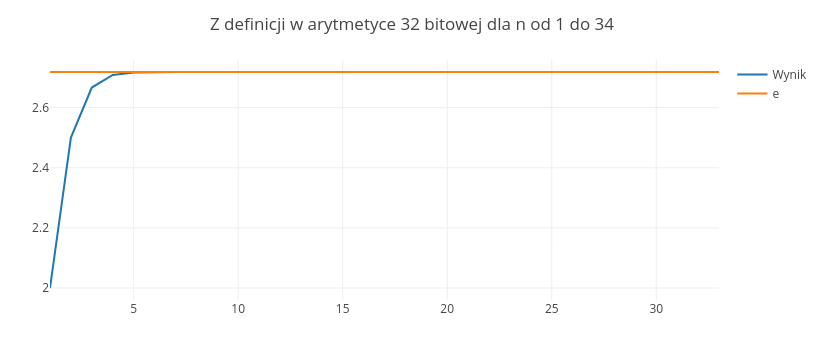
\includegraphics[width=15cm]{d}
  \end{center}
  \caption{Wykres zależności wyniku od $n$ a także porónanie go z wynikiem dokładnym}
  \label{fig:rysunek1}
\end{figure}
\begin{figure}[ht]
  \begin{center}
  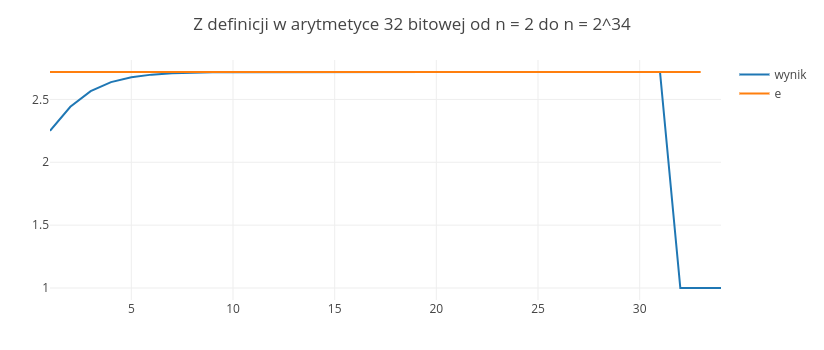
\includegraphics[width=15cm]{d2}
  \end{center}
  \caption{Wykres zależności wyniku od $n$ dla zakresu ukazującego błąd od odpowienio dużych argumentów}
  \label{fig:rysunek2}
\end{figure}


\subsection{Wnioski}
Z wyników tabeli można zauważyć, że różnica maleje dziesięciokrotnie wraz z pomnożeniem liczby $n$ przez 8. Jednakże dla odpowiednio dużych $n$ składnik $\frac{1}{n}$ staje się równy zero przez co $(1+\frac{1}{n})^{n} = (1+0)^{n} = 1^{n} = 1$, co sprawia że metoda ta wymaga bardzo dużo pamięci dla uzyskiwania kolejnych, dokładniejszych przybliżeń, co sprawia, że jest ona nieefektywna.
\newpage
\section{Inne podejście}
\subsection{Opis}
Rozpatrując funkcję $f(x)=e^x$ w $x=1$ otrzymuje się liczbę $e$. Aby móc analizować tą funkcję należy doprowadzić ją do postaci, którą da się zaimplementować na komputerze. Zatem rozwijając $e^x$ w szereg Macloraine'a (a mianowicie jego skończony fragment) w $x=1$ możliwe jest otrzymanie odpowieniego przybliżenia wartości liczby $e$. Więc $e = \sum_{k=0}^{\infty} \frac{1}{k!}$. Jego skończony fragment zaś należałoby przedstawić w postaci $e \approx \sum_{k=0}^{n} \frac{1}{k!}$, odpowiednio zwiększając n możliwe jest zatem uzyskanie odpowiednio dokładnego wyniku.
\subsection{Tabela wyników dla precyzji 16 i 32 bitowej}
\begin{tabular}{||c||c|c|c|c|c|c||} \hline
 & \multicolumn{3}{|c|}{W precyzji 16 bitowej} &\multicolumn{3}{|c|}{W precyzji 32 bitowej}  \\ \hline
N & Wynik & bł. bezwzgl. & bł. wzg. & Wynik & bł. bezwzgl. & bł. wzg.\\ \hline
1 & \textbf{2}.00000 & 7.2e-01  & 2.6e-01 & \textbf{2}.000000000 & 7.2e-01  & 2.6e-01\\
\hline
2  & \textbf{2}.50000  & 2.2e-01  & 8.0e-02 & \textbf{2}.500000000 & 2.2e-01  & 8.0e-02\\
\hline
3  & \textbf{2}.66668  & 5.2e-02  & 1.9e-02 & \textbf{2}.666687011 & 5.2e-02  & 1.9e-02\\
\hline
4  & \textbf{2.7}0837  & 9.9e-03  & 3.6e-03 & \textbf{2.7}08374023 & 9.9e-03  & 3.6e-03\\
\hline
5  & \textbf{2.71}667  & 1.6e-03  & 5.8e-04 & \textbf{2.71}6666666 & 1.6e-03  & 5.9e-04\\
\hline
6  & \textbf{2.718}01  & 2.4e-04  & 9.0e-05 & \textbf{2.718}055555 & 2.3e-04  & 8.3e-05\\
\hline
7  & \textbf{2.7182}6 & 0.0e+00  & 0.0e+00 & \textbf{2.7182}53968 & 2.8e-05  & 1.0e-05\\
\hline
... & ...  & ...  & ...& ...  & ...  & ...\\
\hline
11 & \textbf{2.7182}6 & 0.0e+00  & 0.0e+00 & \textbf{2.71828182}6  & 2.8e-09  & 1.0e-09\\
\hline
12 & \textbf{2.7182}6 & 0.0e+00  & 0.0e+00 & \textbf{2.71828182}7  & 9.3e-10  & 3.4e-10\\
\hline
... & ...  & ...  & ...& ...  & ...  & ...\\
\hline
65  & \textbf{2.7182}6 & 0.0e+00  & 0.0e+00 & \textbf{2.71828182}7  & 9.3e-10  & 3.4e-10\\
\hline
66 & Inf  & -Inf  & -Inf & Inf  & -Inf  & -Inf\\
\hline
\end{tabular}
\subsection{Tabela wyników dla arytemtyki 256 bitowej}
\begin{center}
\begin{tabular}{||c||c|c|c||} \hline
\multicolumn{4}{||c||}{$e \approx \sum_{k=0}^{n} \frac{1}{k!}$ w precyzji 256 bitowej} \\ \hline
N & Wynik & Błąd bezwzględny & Błąd względny\\ \hline
1 & \textbf{2}.0000000000000000  & 7.2e-01  & 2.6e-01\\
\hline
2  & \textbf{2}.5000000000000000  & 2.2e-01  & 8.0e-02\\
\hline
3  & \textbf{2}.6666870117187500  & 5.2e-02  & 1.9e-02\\
\hline
4  & \textbf{2.7}083740234375000  & 9.9e-03  & 3.6e-03\\
\hline
... & ...  & ...  & ...\\
\hline
20  &  \textbf{2.7182818284}590452  & 2.1e-20  & 7.5e-21\\
\hline
21  & \textbf{2.7182818284}590452  & 2.6e-19  & 9.4e-20\\
\hline
... & ...  & ...  & ...\\
\hline
65  & \textbf{2.7182818284}590452  & 1.3e-17  & 4.8e-18\\
\hline
66  & Inf  & -Inf  & -Inf\\
\hline
\end{tabular}
\end{center}
\newpage
\subsection{Wykres}

\begin{figure}[ht]
  \begin{center}
  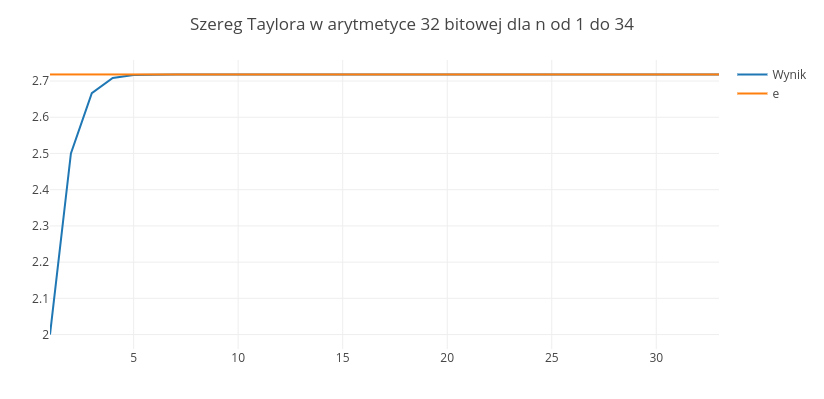
\includegraphics[width=15cm]{sz}
  \end{center}
  \caption{Wykres zależności wyniku przybliżenia $e \approx \sum_{k=0}^{n} \frac{1}{k!}$ od n i zestawienie go z dokładną wartością}
  \label{fig:rysunek}
\end{figure}


\subsection{Wnioski}
Metoda ta (jak można wywnioskować z tabel) jest znacznie szybsza od uzyskiwania liczby $e$ metodą pierwszą a jej błąd dla zadanego $n$ można oszacować z góry przez $(\frac{1}{n!})$ co zostanie udowodnione.
\newtheorem{sad}{Twierdzenie}
\begin{sad}

	Błąd w n-tej sumie szeregu $e \approx \sum_{k=0}^{n} \frac{1}{k!}$ wynosi co najwyżej $\frac{1}{n!}$
\begin{proof}
N-ta reszta szeregu Macloraine'a w postaci Cauchy'ego wynosi $R_{n}(1,0)=\frac{e^{\theta}(1-\theta)^{n}}{n!}$ \hspace{3mm} $\theta \in [0,1]$ badając funkcję $f(\theta) =  e^{\theta}(1-\theta)^{n}$na przedziale do którego należy $\theta$ otrzumujemy:
\newline 
$f'(\theta)= e^{\theta}(1-\theta)^{n-1}(1-\theta-n)$ co jest mniejsze od 0 dla $\theta \in (0,1]$, a zatem największa wartość ta funkcja osiagnie dla $\theta = 0$, więc wyniesie ona 1. Czyli różnica w najgorszym przypadku wynosi $R = \frac{1}{n!}$, skąd jest to oszacowanie błędu z góry.
\end{proof}
\end{sad}
Jest to najszybsza zbieżność jaką udało się uzyskać w tych rozważaniach, jednak pojawia się problem natury numerycznej tak samo jak w przypadku pierwszym, gdyż dla odpowiednio dużych $n$ liczba $\frac{1}{n!}$ może być równa 0, a także poprzez przekroczenie zakresu, prawdopodobnie $n! = 0$ co daje wynik $e \approx \infty$. Aby zniwelować ten błąd w następnej części następuje poprawa (numeryczna) tego sposobu.
\newpage
\section{Próba ulepszenia}
\subsection{Opis}
Tempo zbieżności metody nr 2 można uznać za zadowalające, gdyż chcąc błąd rzędu $10^{-n}$ dla odpowiednio dużych $n$ wystarczy mniej niż $n$ iteracji algorytmu, więc należałoby jedynie uporać się z problemem natury numerycznej dzielenia $\frac{1}{n!}$ co skutkuje:

$e = \sum_{n=0}^{\infty} \frac{1}{n!} =\frac{1}{0!} + \frac{1}{1!} + \frac{1}{2!} + \frac{1}{4!} + \frac{1}{4!} + \frac{1}{5!} ... = 2 + \frac{1}{2}(1 + \frac{1}{3} + \frac{1}{3*4} + \frac{1}{3*4*5!} + ...) =2 + \frac{1}{2}(1 + \frac{1}{3}(1+ \frac{1}{4} + \frac{1}{4*5!} + ...)) = 2 + \frac{1}{2}(1 + \frac{1}{3}(1+ \frac{1}{4}(1 + \frac{1}{5!}(1 + ...))))$
\subsection{Tabela wyników w precyzji 16 bitowej}
\begin{tabular}{||c||c|c|c||} \hline
\multicolumn{4}{||c||}{Wyniki dla $e = 2 + \frac{1}{2}(1 + \frac{1}{3}(1+ \frac{1}{4}(1 + \frac{1}{5!}(1 + ...))))$} \\ \hline
N & Wynik & Błąd bezwzględny & Błąd względny\\ \hline
2 & \textbf{2}.5000000000000000  & 2.2e-01  & 8.0e-02\\
\hline
4 & \textbf{2.7}083129882812500  & 9.9e-03  & 3.7e-03\\
\hline
7 & \textbf{2.7182}617187500000  & 0.0e+00  & 0.0e+00\\
\hline
\end{tabular}
\subsection{Tabela wyników w precyzji 32 bitowej}
%tabela do poparwy przesuniece o 1 iteracje
\begin{tabular}{||c||c|c|c||} \hline
\multicolumn{4}{||c||}{Wyniki dla $e = 2 + \frac{1}{2}(1 + \frac{1}{3}(1+ \frac{1}{4}(1 + \frac{1}{5!}(1 + ...))))$} \\ \hline
N & Wynik & Błąd bezwzględny & Błąd względny\\ \hline
2 & \textbf{2}.5000000000000000  & 2.2e-01  & 8.0e-02\\
\hline
4 & \textbf{2.7}083333330228925  & 9.9e-03  & 3.7e-03\\
\hline
8 & \textbf{2.7182}787694036961  & 3.1e-06  & 1.1e-06\\
\hline
13 & \textbf{2.718281828}7983537  & 0.0e+00  & 0.0e+00\\
\hline
\end{tabular}
\subsection{Tabela wyników w precyzji 256 bitowej}
%tabela do poparwy przesuniece o 1 iteracje
\begin{tabular}{||c||c|c|c||} \hline
\multicolumn{4}{||c||}{Wyniki dla $e = 2 + \frac{1}{2}(1 + \frac{1}{3}(1+ \frac{1}{4}(1 + \frac{1}{5!}(1 + ...))))$} \\ \hline
N & Wynik & Błąd bezwzględny & Błąd względny\\ \hline
2 & \textbf{2}.5000000000000000  & 2.2e-01  & 8.0e-02\\
\hline
4 &  \textbf{2.7}083333333333333  & 9.9e-03  & 3.7e-03\\
\hline
8 & \textbf{2.7182}787698412698  & 3.1e-06  & 1.1e-06\\
\hline
16 & \textbf{2.7182818284}590423  & 3.0e-15  & 1.1e-15\\
\hline
32 & \textbf{2.7182818284}590452  & 1.2e-37  & 4.4e-38\\
\hline
57 & \textbf{2.7182818284}590452  & 0.0e+00  & 0.0e+00\\
\hline
\end{tabular}
\subsection{Wnioski}
Tempo zbieżności tej metody jest takie samo jak w przypadku metody nr 2, jednak przez zamiane sumy na ten schemat udało sie wyeliminować dzielenia przez duże liczby (największy mianownik jaki się pojawi w tym schemacie to $n$) dzięki czemu algorytm przebiega poprzez ciągłę dodawanie 1 i czegoś z przedziału [$\frac{1}{n}$, $1.5$), co wymaga znacznie mniej pamięci niż liczenie $\frac{1}{n!}$.
\newpage
\section{Podsumowanie}
Podsumuwując udało się osiągnąć zerowy błąd w precyzji 16, 32 i 256 bitowej oraz błąd wyrażający się od iteracji algorytmu z rozdzialu 4 (i 3) oszacowany z góry przez $\frac{1}{n!}$.
\newline
\newline
\begin{center}
\begin{tabular}{||c||c|c|c||} \hline
\multicolumn{4}{||c||}{Zestawienie błedów bezwzględnych w precyzji 256 bitowej} \\ \hline
N & $e=(1+\frac{1}{n})^{n}$ & $e = \sum_{n=0}^{\infty} \frac{1}{n!}$ & $e = 2 + \frac{1}{2}(1 + \frac{1}{3}(1+ \frac{1}{4}(...)))$\\ 
\hline
2 & 4.7e-01  & 2.2e-01  & 2.2e-01\\
\hline
4 & 2.8e-01  & 9.9e-03  & 9.9e-03\\
\hline
8 & 1.5e-01  & 3.1e-06  & 3.1e-06\\
\hline
16 & 8.0e-02 & 3.0e-15  & 3.0e-15\\
\hline
$8^5$ & 4.1e-05  & Inf  & 0.0e+00\\
\hline
$8^{10}$ & 1.3e-09 & Inf  & 0.0e+00\\
\hline
\end{tabular}
\end{center}
\begin{figure}[ht]
  \begin{center}
  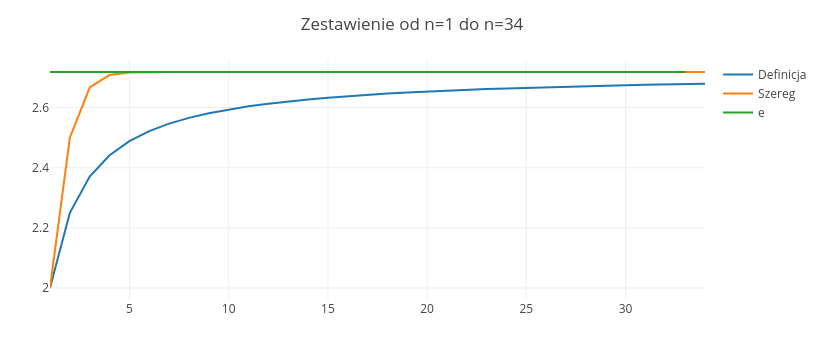
\includegraphics[width=15cm]{z}
  \end{center}
  \caption{Zestawienie wyników metod poruszanych w tym sprawozdaniu}
  \label{fig:rysunek3}
\end{figure}
Porównując wyniki uzyskane w każdej z metod można dojść do wniosku, że metoda poruszona w treści zadania $(e\approx(1+\frac{1}{n})^{n})$ jest skrajnie nieefektywnym sposobem uzyskiwania kolejnych przybliżen liczby e i w rozważanych przypadkach nigdy błąd nie osiągnął zera dla danej precyzji, a także jest zdecydowanie wolniejsza (zmniejsznie błędu 10-cio krotnie na każde przemnożenie $n$ przez 8) niż sposób wyliczenia jej z przekształconego szeregu Macloraine'a ($log_{10}(e-przybliżenie)<-n$ dla odpowiednio dużych n. Wyliczenie przybliżenia liczby $e$ przy pomocy ostatniej metody pozwala także na uzyskanie zerowego błędu w każdej rozważanej precyzji.

\begin{thebibliography}{9}
\itemsep2pt
\bibitem{BM} B. Miś, Tajemnicza liczba e i inne sekrety matematyki,  Wydawnictwo Naukowo-Techniczne, Warszawa 2008

\bibitem{KK}  K. Kuratowski, Rachunek różniczkowy i całkowy, Wydawnictwo naukowe PWN, Warszawa 2018.

\end{thebibliography}

\end{document}
